\section{Data Types}
The following section will describe each data type that {\germinate} can handle in more detail. We will describe both the web interface that is used to display this data as well as what the export formats for each of the types are.

\subsection{Passport Data}
The core data of {\germinate} evolves around accessions and their passport data. Passport data can be described as the sum of all meta-data that relates to the accession.

\begin{figure}
	\centering
	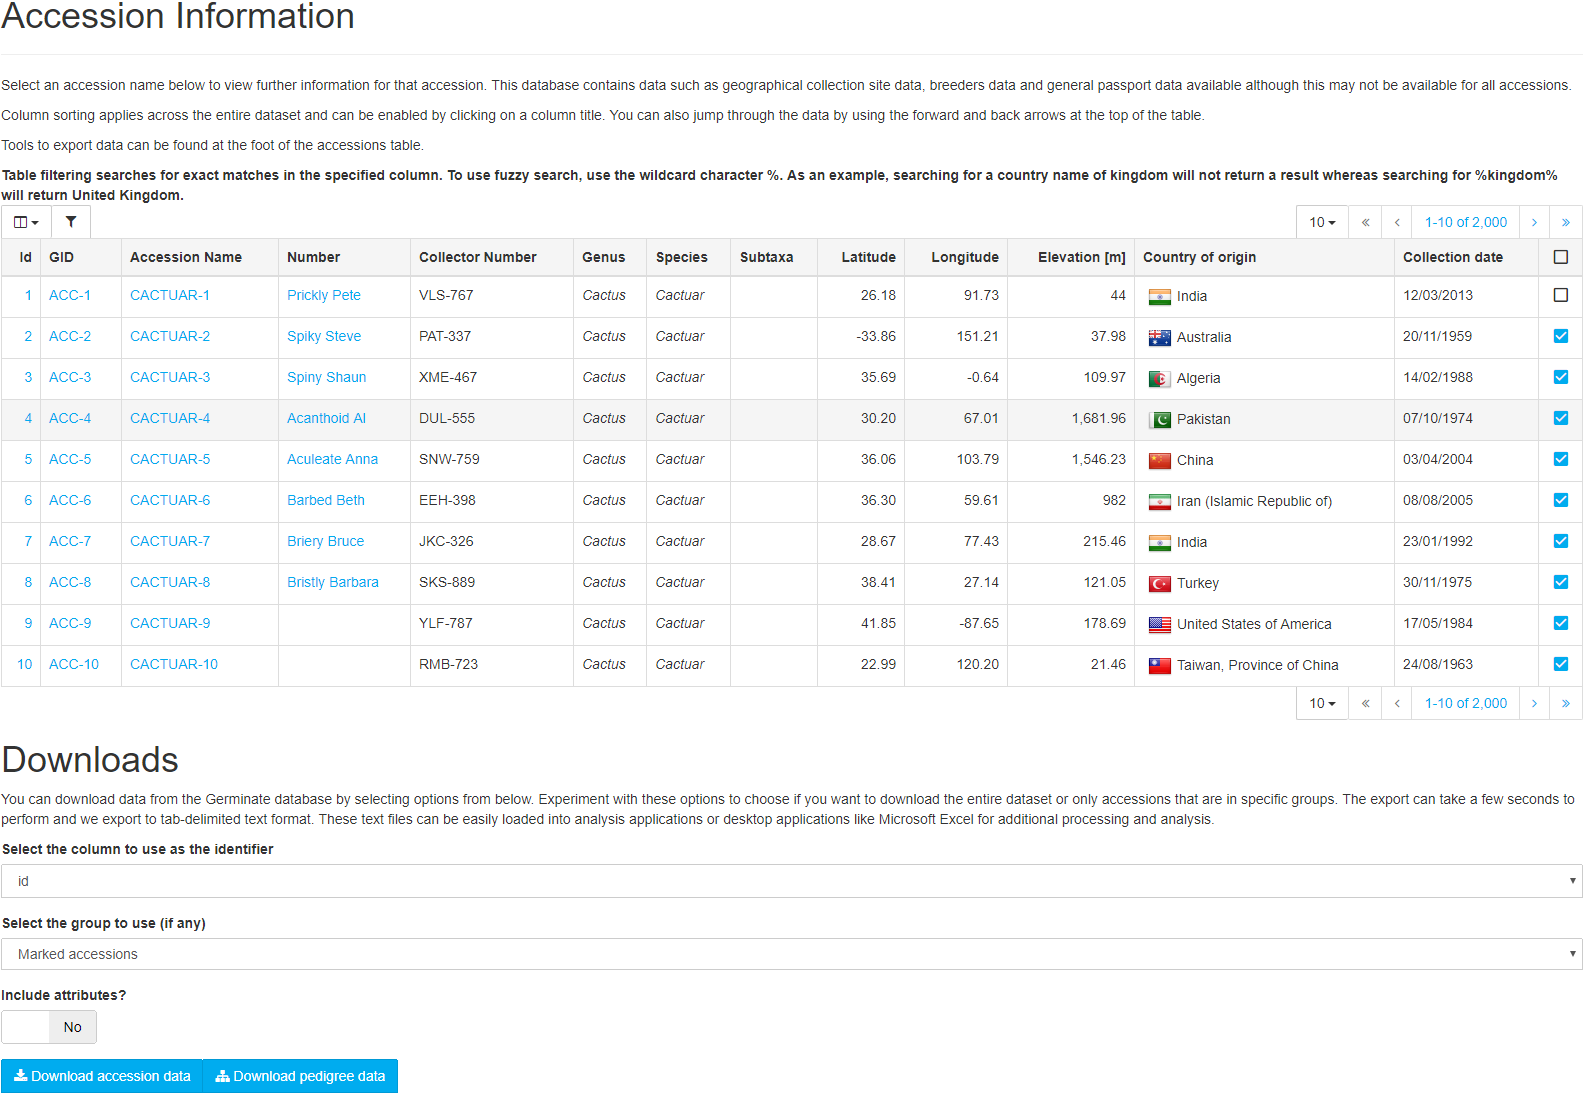
\includegraphics[width=0.85\linewidth]{img/data/accessions.png}
	\caption{The accession overview page shows all the accessions that are part of this {\germinate} instance in a table. This table supports filtering. Accessions can be added to the marked items list by selecting the checkbox in the last column of the table. The download section below the table offers various ways to download data.}
	\label{fig:data:accessions}
\end{figure}

Figure \ref{fig:data:accessions} shows the accession overview page of {\germinate}. The main feature is the table that shows all accessions held in this instance of {\germinate} in a central location. The table supports column sorting and filtering as described in Section \ref{sec:features:filtering} as well as adding accessions of interest to the marked items list (\cf Section \ref{sec:features:marked-items}). The table itself shows the most valuable information about each of the accessions, which is a subset of the Multi-Crop Passport Descriptors (MCPD) \cite{mcpd}.

The MCPD is a widely used international standard to facilitate germplasm passport information exchange defined by the FAO. {\germinate} is fully MCPD V.2.1 compatible. The MCPD standard is used by many genebanks and genetic resources tools and utilities.

The download section located below the table can be used to download the whole set of passport data including accession attributes (\cf Section \ref{sec:data:attributes}) for either the whole dataset, a group or a custom marked item list of accessions. Additionally, the pedigree information for the same constellation of accessions can be downloaded.

Selecting an accession in the table redirects you to the passport data page. This page shows all the information related to a single accession. This includes the MCPD information, holding institute, synonyms, pedigree data, collecting site location, images, groups, datasets, additional attributes and finally there is a section where users can add annotations to this accession (if this feature is enabled available).

\subsection{Pedigree Data}
\label{sec:data:pedigree}

\subsection{Genotypic Data}
When we talk about genotypic data in the context of {\germinate}, we are referring to Single Nucleotide Polymorphic (SNP) or Simple sequence repeat (SSR) data. The data export process is shown in Figure \ref{fig:features:group-subselection}. After selecting the dataset you want to export, you can decide which accessions and markers should be included in the output. Data can be exported against different maps (\cf Section \ref{sec:features:genotypic-maps}), e.g. physical vs. genetic marker positions.

The data is exported into a tab-delimited text format as well as Flapjack \cite{flapjack} format. Figure \ref{fig:features:genotypic-data-flapjack} shows an example of data exported from {\germinate} visualized in Flapjack.

\begin{figure}
	\centering
	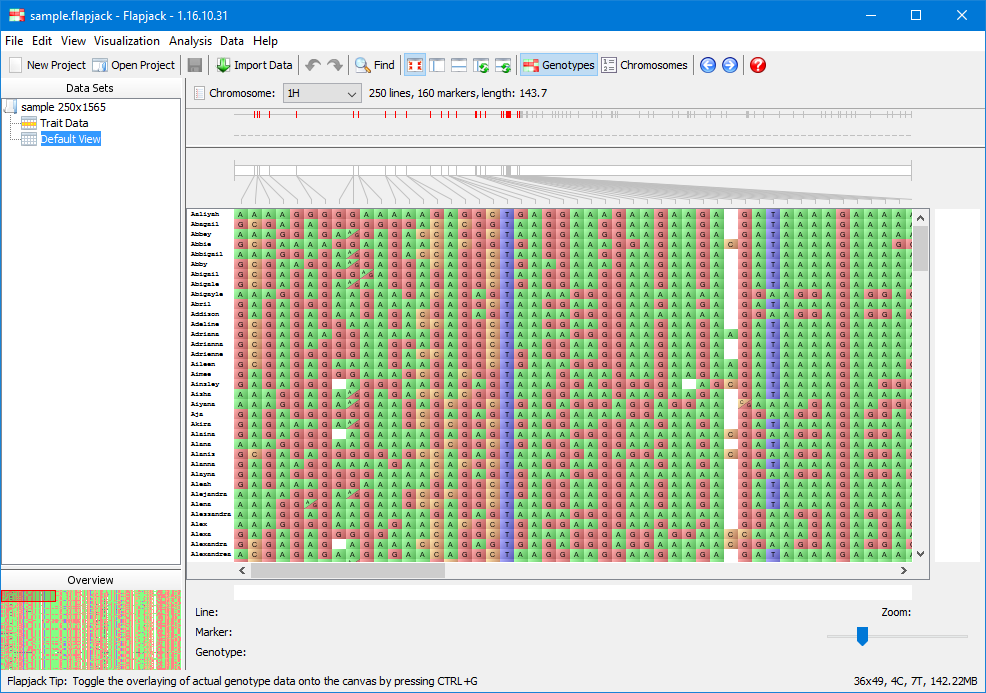
\includegraphics[width=0.85\linewidth]{img/features/genotypic-data-flapjack.png}
	\caption{Genotypic data exported from {\germinate} and visualized in Flapjack.}
	\label{fig:features:genotypic-data-flapjack}
\end{figure}

\subsubsection{Allele Frequency Data}
\todo{Paul}

\subsubsection{Genotypic Maps}
\label{sec:features:genotypic-maps}

\subsubsection{Genetic Markers}

\subsection{Phenotypic Trials Data}
Phenotypic data is a big part of {\germinate}. We put a lot of effort into developing meaningful visualizations as well as functionality and interoperability with our other software tools. 

After selecting a dataset (or multiple datasets), you will have the choice between different visualizations and the data download. The first tab shows an overview over the data within the selected datasets, whereas the second tab lets you plot two phenotypes against each other in a scatter plot. This is particularly useful to see if there is any correlation between them. Hovering over data points shows the values per dimension as well as the accession that is responsible for this data point. Clicking on this data point will take you to the passport page for this accession. You can draw a shape around data points of interest by clicking and dragging the mouse across the chart. This will highlight the data points within the shape. You can then either right-click or use the icon in the top right of the chart to add/remove these items to/from the marked item list.

\subsection{Location Data}
Whether you are interested in geographic locations at which accessions have been collected or where trials have been conducted, location data is one of the central data types in {\germinate} and we put a lot of thought into how we display this information and how we can make it available.

\begin{figure}
	\centering
	\begin{subfigure}[b]{0.47\linewidth}
		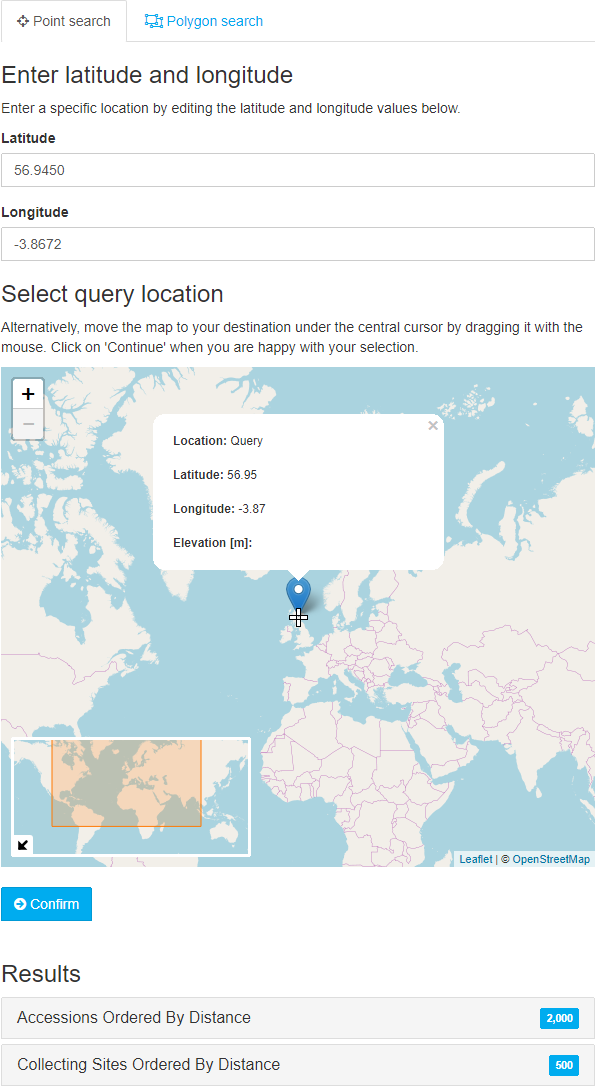
\includegraphics[width=1\linewidth]{img/features/location-search-point.png}
		\caption{Point search}
		\label{fig:features:location-search-point}
	\end{subfigure}
	~
	\begin{subfigure}[b]{0.47\linewidth}
		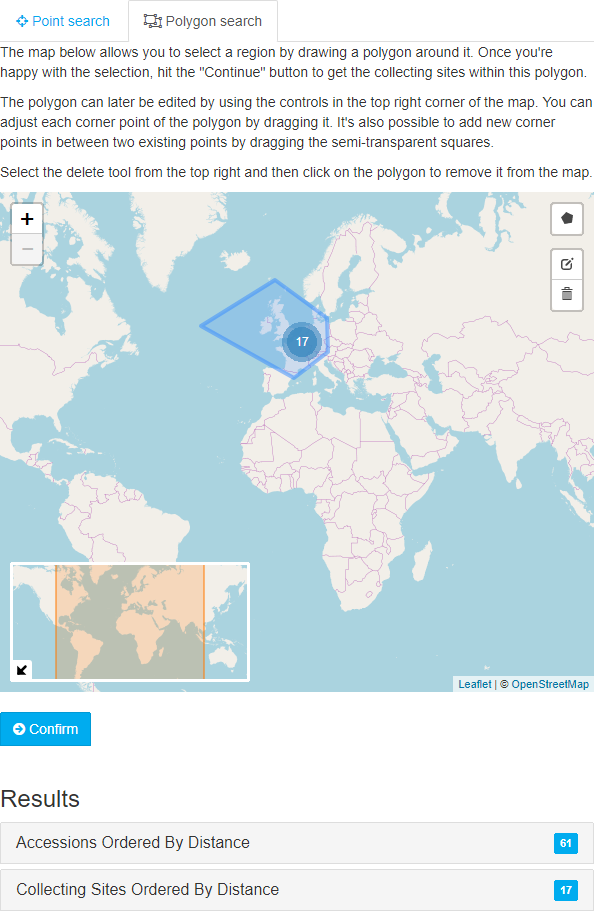
\includegraphics[width=1\linewidth]{img/features/location-search-polygon.png}
		\caption{Polygon search}
		\label{fig:features:location-search-polygon}
	\end{subfigure}
	\caption{The location search interface. The results are shown at the bottom of each page. (A) The point search takes a user-specified query location on the map and returns all accessions and collecting sites ordered by their distance to the query. (B) With the polygon query you can define an arbitrary polygon on the map. {\germinate} will only return items that are located within the specified polygon.}
	\label{fig:features:location-search}
\end{figure}

\begin{figure}
	\centering
	\begin{subfigure}[b]{0.315\linewidth}
		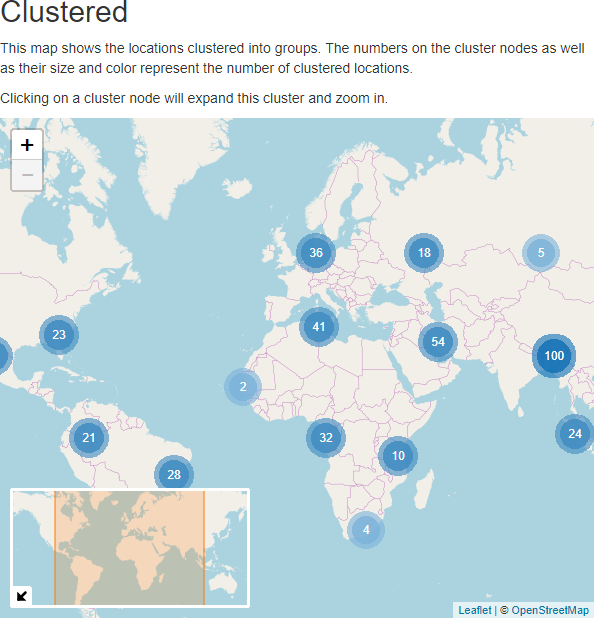
\includegraphics[width=1\linewidth]{img/features/locations-clustered.png}
		\caption{Location clusters}
		\label{fig:features:locations-clustered}
	\end{subfigure}
	~
	\begin{subfigure}[b]{0.315\linewidth}
		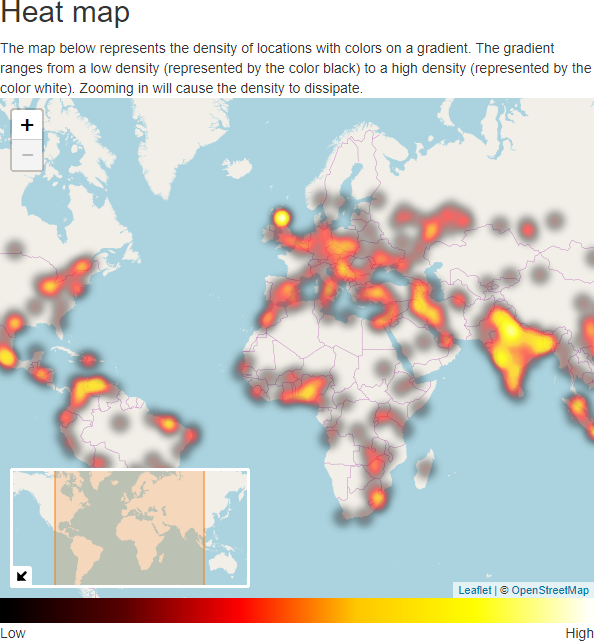
\includegraphics[width=1\linewidth]{img/features/locations-heatmapped.png}
		\caption{Location heat map}
		\label{fig:features:locations-heatmapped}
	\end{subfigure}
	~
	\begin{subfigure}[b]{0.315\linewidth}
		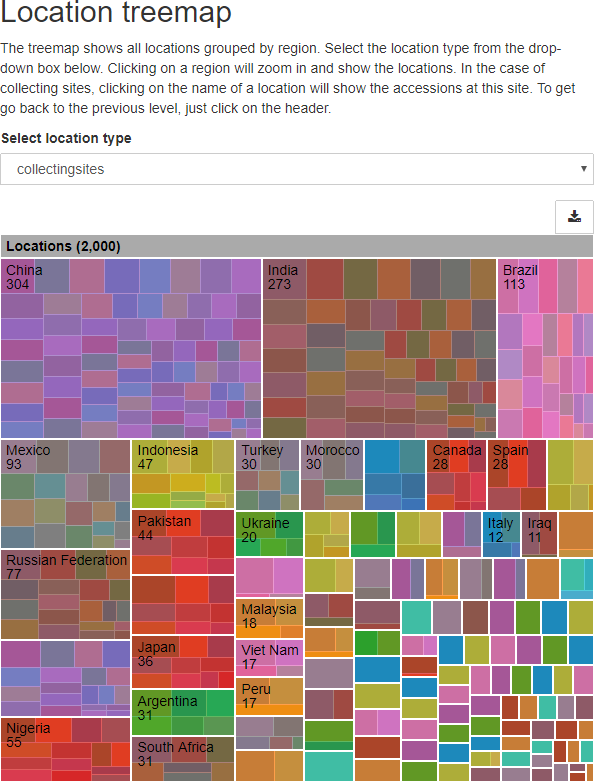
\includegraphics[width=1\linewidth]{img/features/locations-treemapped.png}
		\caption{Location treemap}
		\label{fig:features:locations-treemapped}
	\end{subfigure}
	\caption{Different visualizations of location data on the locations page within {\germinate}. (A) The locations are clustered based on their latitude and longitude. Zooming in will show finer clusters. (B) The heatmap shows the distribution of locations. Yellow and white areas have a high density. (C) The locations are structured in a treemap using the country as the top level. The size of each rectangle represents the number of accessions that have been collected at this site. Selecting any of the countries zooms in to reveal the individual collecting sites.}
	\label{fig:features:locations}
\end{figure}

Location information can be used to filter down accessions by country, region, site name, latitude, longitude or even elevation. The geographic search page allows you to search for accessions or locations based on a point of interest query (Figure \ref{fig:features:location-search-point}) or a custom polygon search (Figure \ref{fig:features:location-search-polygon}). The results are shown below the map grouped into accessions and locations.

The locations page displays the location data in different ways. The locations are clustered in Figure \ref{fig:features:locations-clustered}, visualized utilizing a heat map in Figure \ref{fig:features:locations-heatmapped} and structured in a treemap in Figure \ref{fig:features:locations-treemapped}. All of these visualizations are interactive, so feel free to zoom in and out and select items.

\subsection{Climate Data}

\subsection{Chemical Compound Data}

\subsection{Attribute Data}
\label{sec:data:attributes}